We now create some individuals with the classes and object properties stated in the section above to analyze the reasoner's ability to inter them. We give only a limited set of details to each individual, in the hopes that the reasoner could fill in the holes and show us intuitive relations we thought beforehand.

All the examples created for Plants, Microorganisms, Animals, and Resources are in Tables \ref{tab:plants},\ref{tab:micro}, \ref{tab:res}, and \ref{tab:animals}. We highlight the fact that some properties are clearly missing, like for Oxygen and Water, not clearly stated to be in Savanna. We also mention that the individual Habitat, Savanna, was not programmed with any properties, reason why it's not included in one of the tables.

 
\begin{table}[h!]
    \begin{center}
        \caption{Individuals for plants}
        \begin{tblr}{colspec={|c| c | c|}}
            \hline
            % \multicolumn{4}{|c|}{Plants} \\
            % \hline
            Name& Attributes &Properties\\
            \hline
            { \vspace{0.1in} \\ Acacia}   & {\\ Has fruits\\ Acacia dealbata}    &{Consumes water \\ Found in Savanna \\ Consumes CO2\\ Consumes O2}\\
            \hline
            {Apple} &   {Has fruits \\ Malus domestica}  & {Consumes water}   \\
            \hline
            Grass & & {Consumes CO2 \\ Consumes water}\\
            \hline
        \end{tblr}
        \label{tab:plants}
    \end{center}
\end{table}


 
\begin{table}[h!]
    \begin{center}
        \caption{Individuals for microorganisms}
        \begin{tblr}{colspec={|c| c | c|}}
            \hline
            % \multicolumn{4}{|c|}{Plants} \\
            % \hline
            Name& Attributes &Properties\\
            \hline
            { Bacteria}   & {Escherichia coli}    &{Consumes CO2}\\
            \hline
            {NitroBacteria} &   {Nitrobacter alkalicus}  & {Consumes N2}   \\
            \hline
        \end{tblr}
        \label{tab:micro}
    \end{center}
\end{table}
\newpage
\begin{table}[h!]
    \begin{center}
        \caption{Individuals for resources}
        \begin{tblr}{colspec={|c| c | c|}}
            \hline
            % \multicolumn{4}{|c|}{Plants} \\
            % \hline
            Name& Attributes &Properties\\
            \hline
            {  Carbon Dioxide}   & {CO2}    &{Is in Savanna}\\
            \hline
            {Nitrogen} &   {N2}  & {Is in Savanna}   \\
            \hline
            Oxygen & O2 &\\
            \hline
            Water & H2O &\\
            \hline
        \end{tblr}
        \label{tab:res}
    \end{center}
\end{table}

\begin{table}[h!]
    \begin{center}
        \caption{Individuals for animals}
        \begin{tblr}{colspec={|c| c | c|}}
            \hline
            Name& Attributes &Properties\\
            \hline
            { \\Cow}   & {Weight \\ Bos taurus}    &{Eats grass\\ Consumes water\\ Consumes O2}\\
            \hline
            {\\Giraffe} &   {Weight \\ Giraffa camelopardalis}  & {Eats Acacia\\ Consumes water \\ Consumes O2}\\
            \hline
            {\\Human} & {\\Weight} & {Eats Apple \\ Eats Cow\\ Not eaten by Lion\\ Consumes water\\ Consumes O2}\\
            \hline
            {\\ Lion}& {\\ Weight\\ Panthera leo}&{Eats Giraffe \\ Eats Zebra\\ Found in Savanna\\Consumes water\\ Not eaten by Human }\\
            \hline
            {\\ Zebra}&{\\ Weight \\ Equus quagga} & {Eat Apple\\ Consumes O2\\ Consumes water\\ Eats Grass}\\
            \hline
        \end{tblr}
        \label{tab:animals}
    \end{center}
\end{table}


We now run the reasoner, HermiT, and present some snapshots of the inferences found by it.

\newpage


\subsubsection{Plant Inferences}

We begin with the first two plants in our individual's collection: Acacia and Apple.

\begin{figure}[h!]
    \centering
    \begin{subfigure}[b]{0.8\linewidth}
      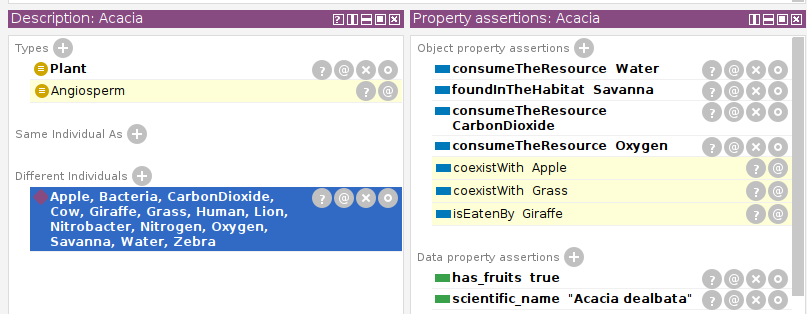
\includegraphics[width=\linewidth]{images/inferences/acacia_inf.png}
      \caption{Acacia's description on Protégé.}
    \end{subfigure}
    \begin{subfigure}[b]{0.8\linewidth}
      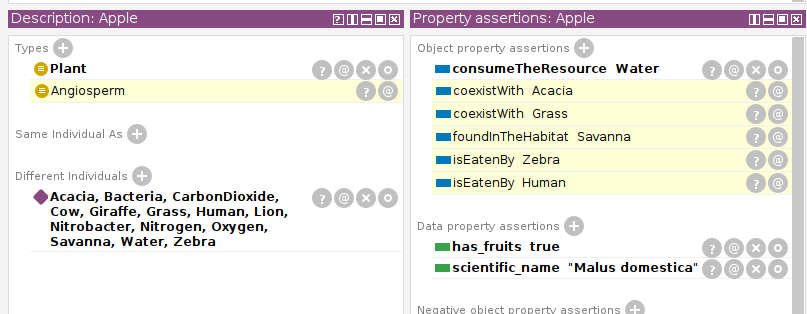
\includegraphics[width=\linewidth]{images/inferences/apple_inf.png}
      \caption{Apple's description on Protégé.}
    \end{subfigure}
    \caption{Inference showcase for both Acacia and Apple individuals of the Plant subclass.}
    \label{fig:acaciaapple_inf}
\end{figure}

  As we can see by \autoref{fig:acaciaapple_inf}, the reasoner is capable of inferring that both plants are Angiosperms, just by the presence of the fruit in their attributes. It's also able to infer their coexistence, between themselves and with Grass, Acacia's property of being eaten by Giraffe, Apple's localization in Savanna and the fact its consumed by both Humans and Zebras.

  In \autoref{fig:grass_inf} we see Grass' inferences for its coexistence with Apple and Apacia, its localization in Savanna, and the fact it's eaten by Zebras and Cows.

  \begin{figure}[h!]
    \centering
    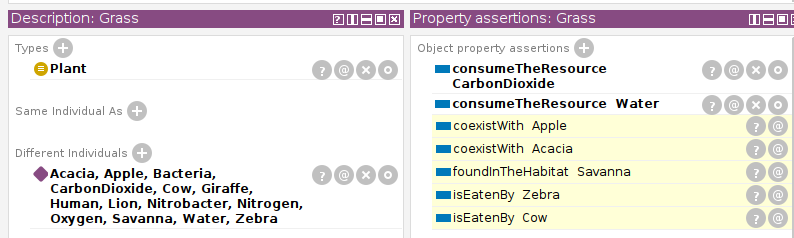
\includegraphics[width=0.8\linewidth]{images/inferences/grass_inf.png}
    \caption{Grass' description on Protégé.}
    \label{fig:grass_inf}
  \end{figure}

  \newpage
  \subsection{Microorganism Inferences}
  For the microorganisms, we check \autoref{fig:micro_inf}. Both of their localization was inferred to be Savannas, and also the fact they coexist, that could be deduced by the fact both consume different resources: Bacteria consumes $CO_{2}$, and NitroBacteria, $N_{2}$.

\begin{figure}[h!]
    \centering
    \begin{subfigure}[b]{0.8\linewidth}
      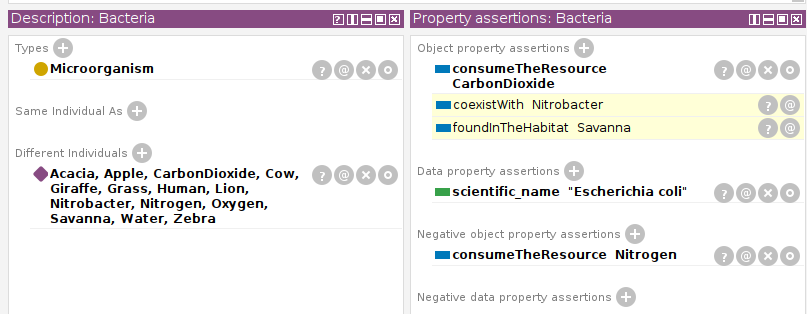
\includegraphics[width=\linewidth]{images/inferences/bac_inf.png}
      \caption{Bacteria's description on Protégé.}
    \end{subfigure}
    \begin{subfigure}[b]{0.8\linewidth}
      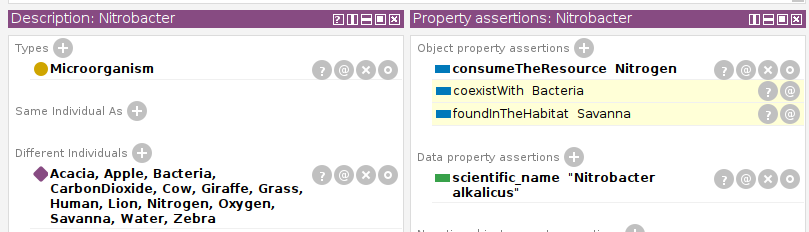
\includegraphics[width=\linewidth]{images/inferences/nitrobac_inf.png}
      \caption{NitroBacteria's description on Protégé.}
    \end{subfigure}
    \caption{Inference showcase for both Bacteria and NitroBacteria individuals of the Microorganism subclass.}
    \label{fig:micro_inf}
\end{figure}

\subsection{Resources inferences}

In \autoref{fig:co2n2_inf}, we see the inferences for Carbon Dioxide($CO_{2}$) and Nitrogen($N_{2}$), which most involves they're being consumed by the right individuals, without explicit mention of those in their properties. For Oxygen($O_{2}$) and water($H_{2}O$), similar inferences are showcased in \autoref{fig:h2oco2_inf}, but now involve a way bigger number of \textit{isConsumedBy} properties, and also the fact they're in Savanna.

\begin{figure}[h!]
    \centering
    \begin{subfigure}[b]{0.8\linewidth}
      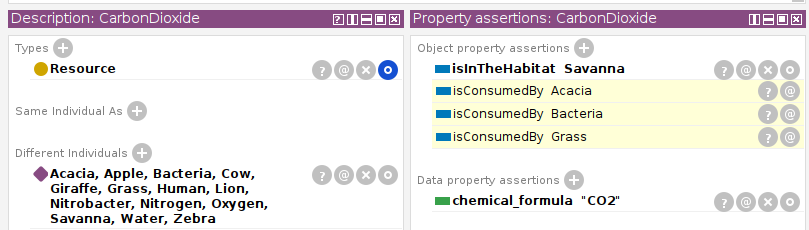
\includegraphics[width=\linewidth]{images/inferences/co2_inf.png}
      \caption{Carbon Dioxide's description on Protégé.}
    \end{subfigure}
    \begin{subfigure}[b]{0.8\linewidth}
      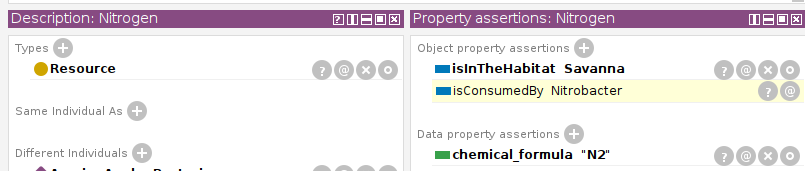
\includegraphics[width=\linewidth]{images/inferences/nitrogen_inf.png}
      \caption{Nitrogen's description on Protégé.}
    \end{subfigure}
    \caption{Inference showcase for both Carbon Dioxide and Nitrogen individuals of the Resource subclass.}
    \label{fig:co2n2_inf}
\end{figure}



\begin{figure}[h!]
    \centering
    \begin{subfigure}[b]{0.8\linewidth}
      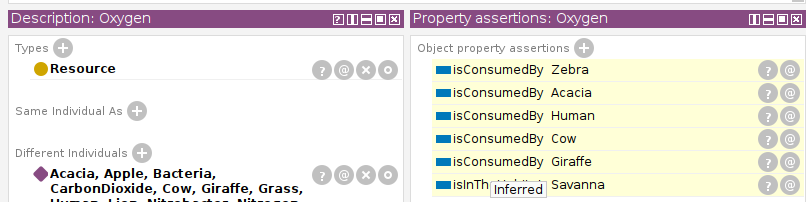
\includegraphics[width=\linewidth]{images/inferences/oxygen_inf.png}
      \caption{Oxygen's description on Protégé.}
    \end{subfigure}
    \begin{subfigure}[b]{0.8\linewidth}
      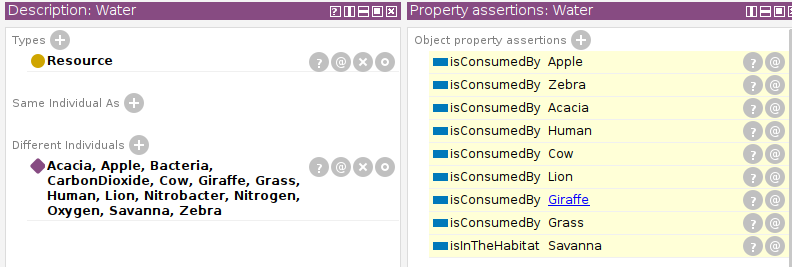
\includegraphics[width=\linewidth]{images/inferences/water_inf.png}
      \caption{Water's description on Protégé.}
    \end{subfigure}
    \caption{Inference showcase for both Oxygen and Water of the Resource subclass.}
    \label{fig:h2oco2_inf}
\end{figure}

\newpage

\subsection{Animals inferences}

We begin by the showcase of our Herbivores inferences, in \autoref{fig:cowzebra_inf}. Aside from the correct coexistence between each other and their predators, the reasoner is also capable of classifying each one of them as \textit{Herbivore}, from the fact they only eat Plants.

\begin{figure}[h!]
    \centering
    \begin{subfigure}[b]{0.8\linewidth}
      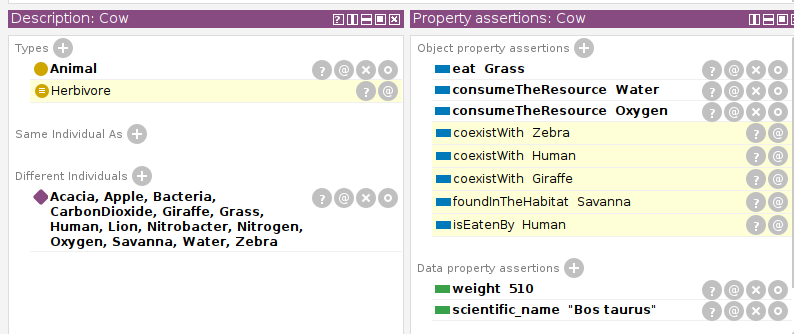
\includegraphics[width=\linewidth]{images/inferences/cow_inf.png}
      \caption{Cow's description on Protégé.}
    \end{subfigure}
    \begin{subfigure}[b]{0.8\linewidth}
      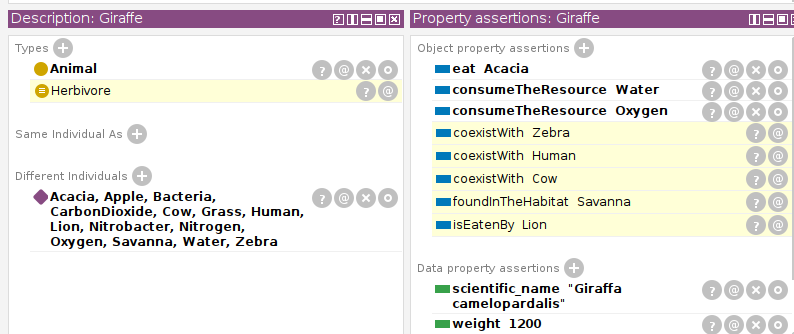
\includegraphics[width=\linewidth]{images/inferences/giraffe_inf.png}
      \caption{Giraffe's description on Protégé.}
    \end{subfigure}
    \begin{subfigure}[b]{0.8\linewidth}
        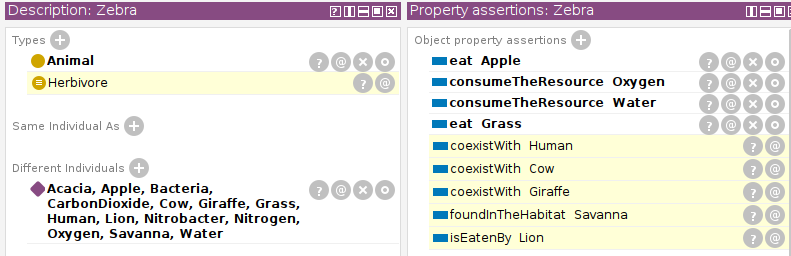
\includegraphics[width=\linewidth]{images/inferences/zebra_inf.png}
        \caption{Zebra's description on Protégé.}
      \end{subfigure}
    \caption{Inference showcase for Cow, Giraffe, and Zebra individuals of the Animal subclass.}
    \label{fig:cowzebra_inf}
\end{figure}

\newpage

Human's and Lion's inferences can be found in \autoref{fig:humanlion_inf}. First we highlight the inference that Lion is a Carnivore from the fact he only eats meat. Second, Human's classification as a Omnivore for the diversity in the resources and Animals it consumes.

\begin{figure}[h!]
    \centering
    \begin{subfigure}[b]{0.8\linewidth}
      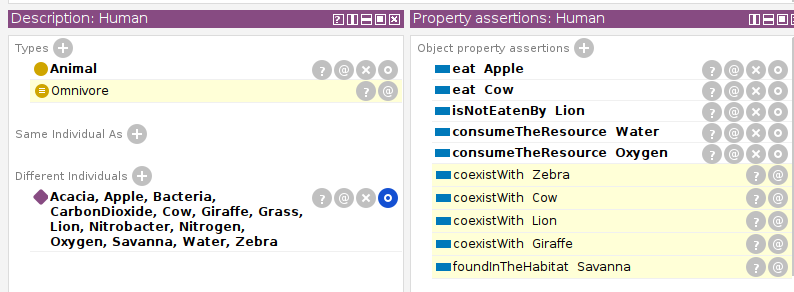
\includegraphics[width=\linewidth]{images/inferences/human_inf.png}
      \caption{Human's description on Protégé.}
    \end{subfigure}
    \begin{subfigure}[b]{0.8\linewidth}
      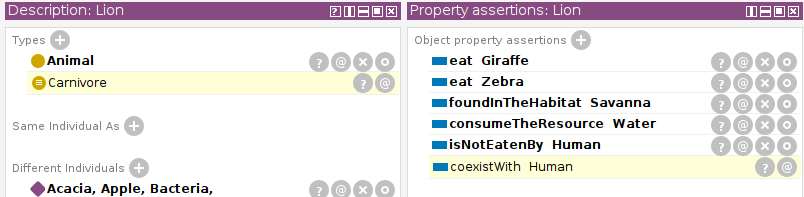
\includegraphics[width=\linewidth]{images/inferences/lion_inf.png}
      \caption{Lion's description on Protégé.}
    \end{subfigure}
    
    \caption{Inference showcase for Human and Lion individuals of the Animal subclass.}
    \label{fig:humanlion_inf}
\end{figure}
